\section{Alterations}

In this case study,the alterations to apply have been identified by considering common perturbations that could occur during image acquisition. It is important to note that the networks used in this study are designed for research purposes and are not intended for a specific application, therefore a precise domain analysis was not possible to perform. The alterations employed are inspired by the work of Arcaini et al. \cite{9176802}. Seven different alteration types are identified, which will be presented in this section. Each alteration is applied on the original test set, where the images pixels are normalized in the range $[0,1]$. For reference, in \Fig~\ref{fig:orig} is shown an example from the original set without any alteration.

\begin{figure}[h]
	\centering
	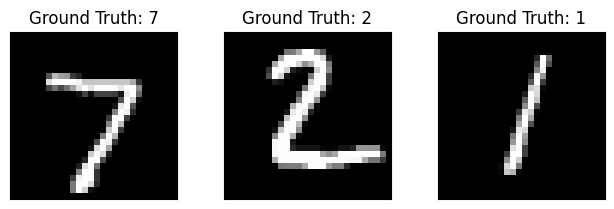
\includegraphics[width=0.6\linewidth]{ImageFiles/Alterations/orig}
	\caption{Images without any alteration}
	\label{fig:orig}
\end{figure}

\subsection{Translation}

This alteration consists in translating all the pixels by a certain amount, which serves as the alteration level in this context. The translation can occur in both vertical and horizontal directions, and when combined, they result in a \textit{rotation}. However, for the purposes of this study, only vertical and horizontal translations will be taken into account. \Fig~\ref{fig:VT} illustrates the effect of vertical translation, while \Fig~\ref{fig:HT} shows an example of the horizontal translation effect.

\begin{figure}[h]
	\centering
	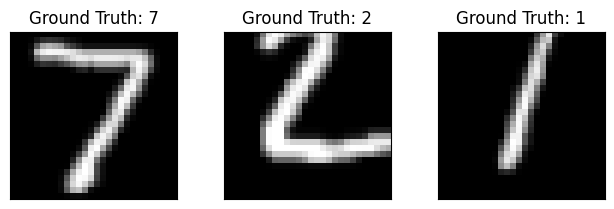
\includegraphics[width=0.6\linewidth]{ImageFiles/Alterations/VT}
	\caption{Example of vertical translation}
	\label{fig:VT}
\end{figure}

\begin{figure}[h]
	\centering
	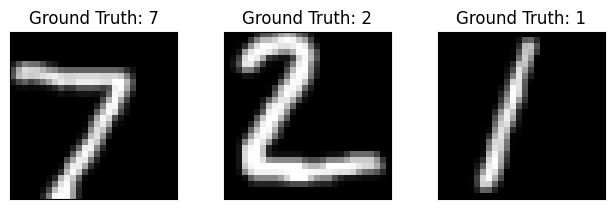
\includegraphics[width=0.6\linewidth]{ImageFiles/Alterations/HT}
	\caption{Example of horizontal translation}
	\label{fig:HT}
\end{figure}

The idea behind this alteration is to replicate situations where the object being detected moves or when the camera is placed incorrectly. The alteration levels evaluated are in the range $[-20,20]$ for both horizontal and vertical translation.

\subsection{Blur}

Blur is an alteration that modifies the sharpness and the scale of an image. It is commonly employed for a variety of purposes, such as simulating motion, reducing noise, or safeguarding sensitive information by obscuring it. This filter effectively eliminates the high-frequency components of an image, similar then to a low-pass filter. In other words, the blur filter applies a Gaussian function to each pixel, considering a specified neighborhood defined by the \textit{radius} value. A higher radius value corresponds to a lower level of detail across the entire image. Therefore, the radius will identify the intensity of this alteration. In particular, the values used in this work fall in the range $[0,2]$. \Fig~\ref{fig:Blur} shows the blur effect.

\begin{figure}[h]
	\centering
	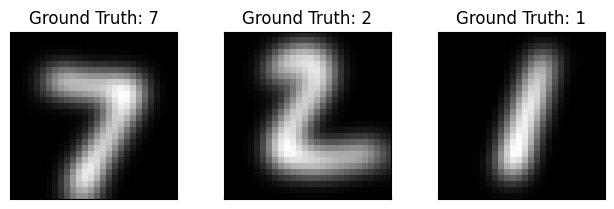
\includegraphics[width=0.6\linewidth]{ImageFiles/Alterations/Blur}
	\caption{Example of blur filter}
	\label{fig:Blur}
\end{figure}

The blur filter allows for the simulation of a camera losing focus, replicating the effect of an out-of-focus shot.

\subsection{Brightness}

Brightness refers to the general level of lightness or darkness within an image. It is one of the fundamental elements of an image quality and it has a substantial impact on the visual appearance and transmission of information in an image. This alteration allows for the simulation of various lighting conditions, which is particularly important when the network operates in an environment where images can come from both light and dark bright setting. The alteration level for brightness is going to be expressed as the relative percentage to the original image brightness level. Negative percentage values indicate a reduction in brightness. The range of alteration values employed falls within the interval of $[-0.5, 0.5]$. \Fig~\ref{fig:Brightness} illustrates the effect of a positive brightness percentage application.

\begin{figure}[h]
	\centering
	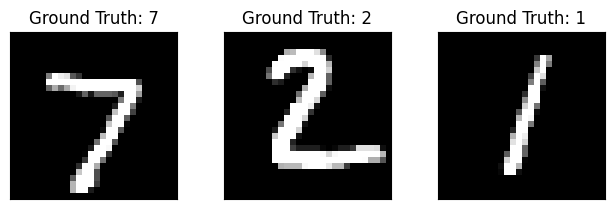
\includegraphics[width=0.6\linewidth]{ImageFiles/Alterations/Brightness}
	\caption{Example of brightness with a positive percentage}
	\label{fig:Brightness}
\end{figure}

\subsection{Zoom}
Zooming involves the action of either enlarging or reducing the size of a specific portion of an image. This enables viewers to concentrate on a particular area of interest within the image, although it may also result in the exclusion of some image portions that could carry important information. \Fig~\ref{fig:Zoom} shows the zoom effect. This alteration crops the image with a certain area, which will be used as alteration level. In particular, it will be expressed in terms of the number of columns and rows cropped. The alteration range used is $[1,2]$, where $1$ identifies the absence of zoom.

\begin{figure}[h]
	\centering
	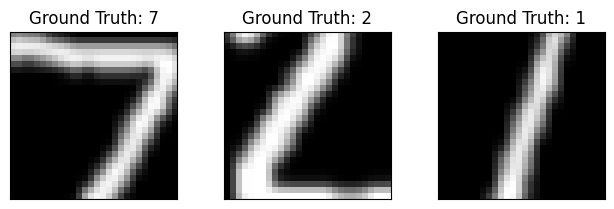
\includegraphics[width=0.6\linewidth]{ImageFiles/Alterations/Zoom}
	\caption{Example of zoom}
	\label{fig:Zoom}
\end{figure}

\subsection{Compression}

Image compression refers to the process of reducing the size of a digital image file while trying to preserve its visual quality and content as much as possible. The primary goal of image compression is to minimize the storage space required for an image, simplifying the tasks of storage, transmission, and efficient display of digital images. Specifically, in this study, the employed method is JPEG compression, which is categorized as a lossy compression technique. In essence, this means that it achieves compression by eliminating certain image data considered less important. This action results in a smaller file size but it can potentially lead to the reduction in image quality, especially when compression is applied at high levels. The alteration level is going to be the compression coefficient, which determines the extent to which the image is compressed. This alteration simulates possible transmission errors, which could lead to a loss of information. In \Fig~\ref{fig:Compression}, an example is presented where the coefficient is set to the maximum value $100$, leading to the loss of all information. The alteration range used is $[0,100]$.

\begin{figure}[h]
	\centering
	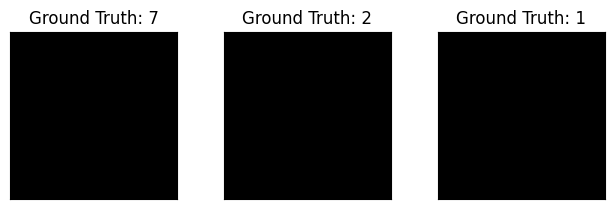
\includegraphics[width=0.6\linewidth]{ImageFiles/Alterations/Compression}
	\caption{Example of compression}
	\label{fig:Compression}
\end{figure}

\subsection{Gaussian noise}

This alteration involves the addition of random noise sampled from a gaussian distribution with a specified variance and zero mean, denoted as $\sigma^2$. This alteration can simulate various types of manipulation errors or interferences that might occur during image acquisition and transmission. The strength of this alteration is controlled by the noise variance, which serves as alteration level. \Fig~\ref{fig:GN} shows how an image changes when random noise is added.

\begin{figure}[h]
	\centering
	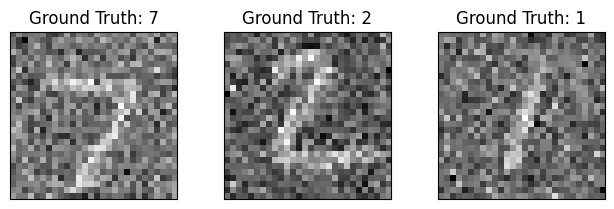
\includegraphics[width=0.6\linewidth]{ImageFiles/Alterations/GN}
	\caption{Example of gaussian noise}
	\label{fig:GN}
\end{figure}

For this alteration the identified range is $[0,0.2]$